\documentclass[12pt]{report}
\usepackage{pdfpages}
\usepackage{lscape}
\usepackage{hyperref}
\hypersetup{
    colorlinks=true,
    linkcolor=black,
    %filecolor=magenta,      
    urlcolor=black,
    breaklinks=true,
   % citecolor=blue,
}
\usepackage[nottoc,notlof,notlot]{tocbibind} 
\usepackage{framed}
\usepackage{rotfloat}
\usepackage{subfig}
\usepackage{graphicx}
\usepackage{caption} 
%\captionsetup[table]{skip=10pt}
\usepackage{graphicx}
\usepackage[utf8]{inputenc}
\usepackage{verbatim}
\usepackage[utf8]{inputenc}
\usepackage{amsmath}
\usepackage[english]{babel}
\usepackage{float}
\usepackage{tikz}
\usepackage{pgfplots}
\pgfplotsset{compat=1.18}
\usepackage{pbox}
\usepackage{url}
\usepackage{tkz-graph}
\usetikzlibrary{arrows}
\usepackage{array}
\usepackage{amssymb}
\providecommand{\checkmark}{\ensuremath{\surd}}
\usepackage{fancyvrb}
\usepackage{listings}
\usepackage{ragged2e}
\usepackage{slashbox}
\makeatletter
\def\BState{\State\hskip-\ALG@thistlm}
\makeatother
\usepackage{sectsty}
\usepackage{comment}
\usepackage{soul}
\usepackage{enumitem}
\usepackage{array}
\usepackage{chngcntr}
\usepackage{cancel}
\usepackage{multirow}
%\usepackage{subfigure}
\usepackage[toc,page]{appendix}
\usepackage{tikz}
\usepackage{setspace}
\usepackage{afterpage}
\usetikzlibrary{shapes,arrows}
\graphicspath{ {images/} }
%\topmargin -23 mm
\providecommand{\keywords}[1]{\textbf{\textit{Keywords---}} #1}
%\headheight 8pt
%\oddsidemargin 0mm
%\evensidemargin -5mm
\textwidth 161mm
\textheight 210mm
\linespread{1}
%\footskip = 60pt
\usepackage{titlesec}
\chapterfont{\centering}
\newcolumntype{P}[1]{>{\centering\arraybackslash}p{#1}}
\newcolumntype{M}[1]{>{\centering\arraybackslash}m{#1}}
\renewcommand{\baselinestretch}{1.3} 
\titleformat{\chapter}[display]   
{\normalfont\huge\bfseries\centering}{\chaptertitlename\ \thechapter}{10pt}{\Huge\centering}   
\titlespacing*{\chapter}{0pt}{-50pt}{5pt}
\usepackage{pdfpages}
\usepackage[linesnumbered,ruled]{algorithm2e}
\usepackage[  
 top    = 1.5in,
  bottom = 1in,
  left   = 1.5in,
  right  = 1in, 
  %headsep=5mm,%%% Example
  %includeheadfoot%%%%%%%%%%%%%%%%%%%%%%%%%%
  ]{geometry}
%below code used for page bordering
\iffalse
\usepackage{pgf}
\usepackage{pgfpages}0
\pgfpagesdeclarelayout{boxed}
{
  \edef\pgfpageoptionborder{4pt}
}
{
  \pgfpagesphysicalpageoptions
  {%
    logical pages=1,%
  }
  \pgfpageslogicalpageoptions{1}
  {
    border code=\pgfsetlinewidth{1.5pt}\pgfstroke,%
    border shrink=\pgfpageoptionborder,%
    resized width=.95\pgfphysicalwidth,%
    resized height=.95\pgfphysicalheight,%
    center=\pgfpoint{.5\pgfphysicalwidth}{.5\pgfphysicalheight}%
  }%
}
\pgfpagesuselayout{boxed}
\setlength{\parindent}{2cm}
\usetikzlibrary{calc}
\usepackage{eso-pic}
\fi

\begin{document}
\counterwithin{table}{section}
\counterwithin{figure}{section}
\thispagestyle{empty}
\iffalse
\AddToShipoutPictureBG*{%
\begin{tikzpicture}[overlay,remember picture]
\draw[line width=4pt]
    ($ (current page.north west) + (1cm,-1cm) $)
    rectangle
    ($ (current page.south east) + (-1cm,1cm) $);
\draw[line width=1.5pt]
    ($ (current page.north west) + (1.2cm,-1.2cm) $)
    rectangle
    ($ (current page.south east) + (-1.2cm,1.2cm) $);
\end{tikzpicture}
}
\fi
 \begin{center}
	Major Project Report on\\
	\null
	\textbf{\large \textbf{ADAPTIVE-ORDER STATE TRANSITIONS IN LINEAR RNNs FOR EFFICIENT STATE TRACKING}}\\
	\null
	
	Submitted in partial fulfillment of the requirements for the degree of\\
	\null
	BACHELOR OF TECHNOLOGY\\
	in\\
	ARTIFICIAL INTELLIGENCE\\
		by \\
	\textbf{Utkarsh Shukla (Roll No.)}\\
	\vspace{0.8em}
	\large{\textit{under the guidance of}} \\
	\vspace{0.8em}
	
	\large{\textbf{Anand Kumar M}}\\
	\begin{figure}[h] % b - bottom, t - top, h - here
		\centering{
			
\includegraphics[width=6cm, height=6cm]{symbol.jpg}
		}
	\end{figure}
DEPARTMENT OF INFORMATION TECHNOLOGY\\
NATIONAL INSTITUTE OF TECHNOLOGY KARNATAKA\\
SURATHKAL, MANGALORE - 575025\\
SEPTEMBER, 2026\\
\end{center}
\clearpage
\thispagestyle{empty}


\begin{framed}
	\begin{center}
		\textbf{{\Large DECLARATION}}\\
	\end{center}
	\null
	I/We hereby \textit{declare} that the Project Work Report entitled \textit{\textbf{"Adaptive-Order State Transitions in Linear RNNs for Efficient State Tracking"} },  which is being submitted to the \textbf{National Institute of Technology Karnataka, Surathkal}, for the award of the Degree of Bachelor of Technology in Artificial Intelligence, is a \textit{bonafide report of the work carried out by me/us.} The material contained in this Project Report has not been submitted to any University or Institution for the award of any degree.
	\\
	\\
	\textit{Name of the Student (Registration Number) with Signature }
	\begin{enumerate}[label={(\arabic*)}]
		\item  Utkarsh Shukla (Roll No.)
	\end{enumerate}
	\null
	Department of Information Technology \\
	Place     : NITK, Surathkal-575025 \\
	Date      : DD/MM/YYYY 
	\\
	\\
	\\
	\\
	\\
	\\
	\\
	\\
	\\
	\\
\end{framed}
\clearpage

\begin{framed}
	\begin{center}
		\textbf{{\Large CERTIFICATE}}
	\end{center}
	\null
	This is to \textit{certify} that the Project Work Report entitled \textit{\textbf{"Adaptive-Order State Transitions in Linear RNNs for Efficient State Tracking"}} submitted by \\
	\\
	\textit{Name of the Student (Registration Number)}
	\begin{enumerate}[label={(\arabic*)}]
		\item  Utkarsh Shukla (Roll No.)
	\end{enumerate}
	as the record of the work carried out by him/her/them, is \textit{accepted as the B.Tech. Project work report submission} in partial fulfillment of the requirement for the award of the degree of \textbf {Bachelor of Technology} in Artificial Intelligence.
	\\
    \\
	\begin{minipage}{14cm}
		\begin{center}                                      	\vspace{1.5cm}	
			\textbf{Signature of Major Project Guide with date}
            \\Anand Kumar M
            \\Write the designation of the Major Project Guide here \\
			Department of Information Technology, NITK Surathkal \\
			\end{center}       
     \vspace{0.75cm}
        \begin{center}                                      	\vspace{1.5cm}	
			\textbf{Chairman - DUGC}
            \\{Signature with Date and Seal}
          	\end{center} 
	\end{minipage}
\\
\\
\\
\\
\\
\end{framed}
\thispagestyle{empty}
\clearpage

\thispagestyle{empty}
\clearpage
\begin{center}
	\textbf{{\Large ACKNOWLEDGEMENT}}\\
    \thispagestyle{empty}
\end{center}
\justifying
I would like to express my sincere gratitude to my project guide, \textbf{Anand Kumar M}, for his guidance, encouragement and critical feedback throughout this work. I also thank the Department of Information Technology, National Institute of Technology Karnataka, Surathkal, for providing the academic environment and resources that made this project possible.

I am grateful to the authors of DeltaProduct and of the \texttt{flash-linear-attention} library for releasing their code openly, which made it possible to reproduce and extend their work on modest hardware.
\vspace{2cm}

\hfill Utkarsh Shukla
\thispagestyle{empty}
\clearpage


\pagenumbering{roman}
\begin{center}
\textbf{{\Large ABSTRACT}}\\
\begin{center}
\justifying
Linear recurrent networks attain inference cost linear in sequence length, but have historically been weak at state tracking, the task of maintaining a structured hidden state whose correct value depends on the entire preceding input. Recent work closes much of this gap by constructing each state-transition matrix as a product of $n_h$ generalized Householder factors, where a larger $n_h$ yields a richer set of reachable transitions at proportionally greater computational cost. In existing formulations $n_h$ is a single global hyperparameter, fixed before training and applied identically to every token.

This work establishes that the number of Householder factors a symbol requires is not a property of that symbol. It is determined by the algebraic closure of the entire input alphabet, through the minimum dimension of a faithful representation of the group that the alphabet generates. The resulting order-requirement model is verified by explicit construction in double precision: a five-cycle requires four factors when the alphabet generates the symmetric group $S_5$, and only two when the alphabet generates the alternating group $A_5$, which admits a three-dimensional faithful representation. A direct consequence is that introducing a single transposition, the least expressive symbol available, doubles the requirement of every five-cycle in the alphabet. Two hard bounds on reachability are also established: a rank bound that forces the factor count to be at least the transposition length of the target permutation, and a determinant-parity bound that governs the admissible padding of shorter solutions.

Building on this analysis, an adaptive-order layer is proposed in which a monotone halting gate assigns a per-token factor count, trained end to end with a penalty on expected computation and no supervision on the allocation itself. Under an oracle allocation, in which the correct per-token order is supplied from ground truth, the layer attains accuracy above $0.9997$ at $1.15$ to $1.75$ factors per token on alphabets where the cheapest adequate fixed order costs four, a reduction in required work of $2.29\times$ to $3.48\times$. Trained end to end across three random seeds, the halting gate reproduced the oracle allocation exactly in one seed, assigning one factor to every low-requirement token and four to every high-requirement token over $256{,}000$ evaluated tokens with zero mean absolute allocation error. A supporting stability analysis over fifty training runs establishes that outcomes on the harder alphabets are bimodal rather than concentrated, and that the configurations in which adaptive order offers the largest reduction are precisely those that train reliably.
\end{center}
\end{center}
\keywords{Linear recurrent networks, state tracking, Householder transformations, adaptive computation, group representations, conditional computation}\\

\renewcommand*{\contentsname}{\MakeUppercase{Contents}}
\renewcommand*{\listfigurename}{\MakeUppercase{List of Figures}}
\renewcommand*{\listtablename}{\MakeUppercase{List of Tables}}
\renewcommand{\bibname}{REFERENCES}
\tableofcontents
\clearpage

\begingroup
\addcontentsline{toc}{chapter}{LIST OF FIGURES}
\listoffigures
\clearpage
\endgroup

\begingroup
\addcontentsline{toc}{chapter}{LIST OF TABLES}
\listoftables
\clearpage
\endgroup

\renewcommand{\chaptername}{CHAPTER}
% ===================================================Chapter 1===============================================================
\chapter{INTRODUCTION}
\section{Overview}
\pagenumbering{arabic}

A sequence model performs \emph{state tracking} when it maintains a structured
internal quantity whose correct value at position $t$ depends on every symbol
observed before it. Tracking the configuration of a board across a sequence of
moves, the value of a variable across a program trace, or the orientation of a
rigid body across a stream of rotations are all instances of the same
computational pattern. Attention-based architectures address it by re-reading the
entire history at every position, which costs time quadratic in sequence length
\cite{attention}. Linear recurrent architectures, including linear attention
\cite{lineartransformers}, structured state-space models \cite{s4, mamba}, and
the delta-rule family \cite{fastweight, deltanet}, instead carry a fixed-size
state forward and therefore achieve cost linear in length. This efficiency has
historically come at the expense of exactly the capability described above:
models whose state-transition operator is diagonal are provably unable to track
non-commutative structure \cite{illusionofstate, diagonalssm}.

Permutation-group word problems are the standard probe for this capability. The
model receives a sequence of group elements and must emit, at every position, the
cumulative product of all elements seen so far. The task admits no shortcut, its
correct answer is computable exactly, and its difficulty can be varied in a
controlled manner by changing the alphabet of group elements from which sequences
are drawn.

The DeltaProduct layer \cite{deltaproduct} narrows the gap between linear cost
and state-tracking capability by constructing each state-transition matrix as a
product of $n_h$ generalized Householder factors,
\begin{equation}
A_t \;=\; \prod_{i=1}^{n_h} \bigl( I - \beta_{t,i}\, k_{t,i} k_{t,i}^{\!\top} \bigr),
\qquad \lVert k_{t,i} \rVert = 1, \quad \beta_{t,i} \in [0,2].
\label{eq:deltaproduct}
\end{equation}
Each factor is a rank-one modification of the identity, and the number of such
factors controls the expressivity of the set of transitions the layer can
realise. Increasing $n_h$ enlarges that set and increases computation in direct
proportion. In the formulation as published, $n_h$ is a single global
hyperparameter: it is chosen once, before training, and the same number of
factors is applied to every token of every sequence.

This work is concerned with that design decision. It establishes what the correct
per-token factor count is, shows that this quantity cannot be read off individual
tokens, and develops a layer in which the count is predicted per token by a
learned halting gate trained under a penalty on expected computation.

\section{Motivation}

The immediate argument for a per-token factor count is one of efficiency. On a
sequence in which most symbols require a single factor and a minority require
four, a fixed-order model must be provisioned for the maximum and therefore pays
that maximum everywhere. Allocating per token reduces the required work to the
expected requirement rather than its supremum, and the reduction is larger the
more skewed the distribution of requirements.

A second and stronger argument follows from the analysis developed in this work.
The number of Householder factors that a symbol requires is not a property of the
symbol. It is a property of the algebraic closure of the entire alphabet from
which symbols are drawn. A layer is free to realise any faithful representation
of the group generated by the alphabet, and the factor count required for a given
element is the rank of that element's deviation from the identity, minimised over
all such representations. The consequence is concrete and counter-intuitive:
adding a single transposition to an alphabet of five-cycles changes the generated
group from the alternating group $A_5$ to the symmetric group $S_5$, removes
access to the three-dimensional faithful representation that $A_5$ admits, and
thereby doubles the requirement of every five-cycle in the alphabet, from two
factors to four. The least expressive symbol available makes every other symbol
more expensive.

This has a practical implication for the hyperparameter itself. Selecting $n_h$
correctly requires knowing the minimum faithful representation dimension of the
group generated by the data, a quantity that is not available from inspection of
a dataset and that changes discontinuously when the alphabet changes. A
practitioner who fixes $n_h$ globally must therefore over-provision, wasting
computation on every token, or under-provision, in which case the layer cannot
represent the required transitions and the failure is silent. A layer that infers
its own order removes a hyperparameter that cannot be set reliably by hand, and
this argument is independent of any efficiency gain.

A third consideration concerns measurement. The training behaviour of these
architectures on the harder alphabets is bimodal rather than concentrated: a run
either escapes an extended loss plateau and solves the task, or remains at chance
accuracy, with intermediate outcomes rare. Conclusions drawn from single training
runs on such configurations are therefore unreliable, and the experimental
protocol adopted here reports escape fractions over repeated runs in place of
point estimates wherever this behaviour is present.

\section{Contributions}

The contributions of this work are the following.

\begin{enumerate}[label={(\arabic*)}]
	\item An order-requirement model for Householder-product state transitions,
	establishing that the factor count required by a symbol is determined by the
	minimum faithful representation dimension of the group generated by the whole
	alphabet, together with its verification by explicit construction in double
	precision.
	\item Two reachability bounds for products of generalized Householder factors:
	a rank bound relating the factor count to the transposition length of the
	target permutation, and a determinant-parity bound that determines when a
	shorter solution may be padded to a longer factor count. The second bound
	constrains the design of any gating mechanism applied to such a layer.
	\item An adaptive-order layer in which a monotone halting gate predicts a
	per-token factor count, trained end to end with a penalty on expected
	computation and without supervision on the allocation.
	\item An empirical characterisation of capability at matched computation,
	quantifying the reduction in required work that a correct per-token allocation
	achieves relative to the cheapest adequate fixed order.
	\item A stability analysis over fifty training runs establishing the bimodal
	character of training outcomes on these tasks, and the measurement protocol
	that follows from it.
\end{enumerate}

% ===================================================Chapter 2===============================================================
\begin{center}
	\chapter{LITERATURE REVIEW}
\end{center}
\justifying

\section{Background and Related Works}

\subsection{Linear recurrent architectures}

Attention computes, at every position, a weighted combination over the entire
preceding sequence, giving cost quadratic in sequence length \cite{attention}.
Linear attention replaces the softmax with a kernel feature map, which allows the
summation to be reorganised into a recurrence over a fixed-size state and reduces
the cost to linear \cite{lineartransformers}. Schlag et al. \cite{fastweight}
subsequently identified this recurrence as a form of fast weight programming and
observed that the elementary additive update overwrites capacity as the sequence
lengthens, motivating an update rule with an explicit removal term.

Structured state-space models arrive at a similar recurrence from a different
direction, parameterising a linear dynamical system whose transition operator is
diagonal or diagonal-plus-low-rank \cite{s4}, with selective, input-dependent
parameterisations following later \cite{mamba}. Gated linear attention
\cite{gla} introduces data-dependent decay into the linear-attention recurrence
and supplies hardware-efficient chunked kernels for training it at scale.

\subsection{State tracking and its limits}

The capability that separates these architectures is state tracking. Merrill et
al. \cite{illusionofstate} show that state-space models whose transition operator
is diagonal cannot express the composition of non-commuting operations, placing
them below the complexity class required for permutation tracking regardless of
depth or width. Shakerinava et al. \cite{diagonalssm} refine this
characterisation for input-dependent complex-valued diagonal models, and report
in addition that multi-layer models frequently fail to learn state tracking for
non-Abelian groups even in configurations where they possess the representational
capacity to express it, indicating a gap between expressivity and optimisation.
Liu et al. \cite{shortcuts} establish the complementary result for
attention-based models, showing that shallow transformers learn shortcut
solutions to automata that generalise poorly beyond the training length.

Permutation-group word problems are the standard instrument in this line of work.
Sequences are drawn from an alphabet of permutations and the target at each
position is the running product. The symmetric group $S_5$ is the usual hard
case, since it is non-solvable and therefore lies outside what a constant number
of diagonal layers can express.

\subsection{Householder products as transition operators}

DeltaNet \cite{deltanet} makes the delta-rule recurrence parallelisable over
sequence length by expressing a chunk of updates as a matrix product, which
yields a state-transition operator that is a product of rank-one modifications of
the identity. DeltaProduct \cite{deltaproduct} generalises this by taking $n_h$
such factors per token, each a generalized Householder transformation
$H(\beta,k) = I - \beta k k^{\!\top}$ with $\lVert k \rVert = 1$ and
$\beta \in [0,2]$. The parameter $\beta$ interpolates between three regimes: at
$\beta = 0$ the factor is the identity, at $\beta = 1$ it is the orthogonal
projection removing the component along $k$, and at $\beta = 2$ it is the
reflection in the hyperplane orthogonal to $k$. Since a transposition of two
coordinates is precisely such a reflection, a permutation expressible as a
product of $\ell$ transpositions is realisable by $\ell$ reflection factors, and
DeltaProduct accordingly reports that state-tracking performance on $S_n$
improves as $n_h$ is raised towards the maximum transposition length. The number
of factors is a global hyperparameter, and the paper identifies per-token
adaptive order as an open direction.

\subsection{Adaptive computation}

Allocating a variable amount of computation per input is a well-established
mechanism. Adaptive Computation Time \cite{act} attaches a halting unit to a
recurrent step, accumulates halting probabilities until they exceed a threshold,
and penalises the expected number of steps through a ponder cost. PonderNet
\cite{pondernet} reformulates the halting distribution probabilistically and
supplies an unbiased gradient estimator with improved stability. Universal
Transformers \cite{universaltransformer} apply the same principle to depth in an
attention model. These mechanisms are mature and are adopted here without
modification; the contribution of the present work lies elsewhere.

\section{Outcome of Literature Review}

Table \ref{table:survey} summarises the surveyed works along the two axes
relevant to this project: whether the architecture can express non-commutative
state transitions, and whether the computation it spends per token is fixed or
variable.

\begin{table}[ht]
	\caption{Position of the surveyed architectures} % title of Table
	\centering
	\begin{tabular}{P{4.6cm} P{3.4cm} P{3.4cm}}
		\hline\hline
		Architecture family & Non-commutative state tracking & Computation per token \\ [0.5ex]
		\hline
		Softmax attention \cite{attention} & yes, at quadratic cost & fixed \\
		Linear attention \cite{lineartransformers, gla} & no & fixed \\
		Diagonal state-space models \cite{s4, mamba} & no \cite{illusionofstate} & fixed \\
		Delta rule \cite{fastweight, deltanet} & limited, one factor & fixed \\
		Householder products \cite{deltaproduct} & yes, for $n_h$ sufficiently large & fixed, global $n_h$ \\
		Adaptive computation \cite{act, pondernet} & not applicable & variable \\ [1ex]
		\hline
	\end{tabular}
	\label{table:survey}
\end{table}

Three observations follow from the survey.

First, the expressivity question for this architecture family is settled in
outline. Diagonal transition operators cannot track non-commutative structure,
products of rank-one modifications can, and the factor count governs how much
structure is reachable. What has not been established is the correct value of
that count for a given task, as distinct from the observation that larger values
perform better.

Second, the cost accounting in this line of work treats the required expressivity
as an attribute of the individual symbol, through the identification of the
factor count with the transposition length of the corresponding permutation. This
identification is exact for the standard representation of a symmetric group, but
it is not exact in general, and the discrepancy is not incidental. Chapter 3
establishes that the requirement is determined by the group generated by the
whole alphabet, and that the same symbol may require two factors under one
alphabet and four under another.

Third, adaptive computation supplies a mature halting mechanism that can be
applied without modification. The open question is therefore not how a model
should halt, but what the correct allocation is and whether it can be inferred
from the task without supervision.

\section{Problem Statement}

In linear recurrent architectures whose state-transition operator is a product of
generalized Householder factors, the number of factors per token, $n_h$, is a
global hyperparameter applied uniformly to every input symbol. The expressivity
actually required varies across symbols, so a model with a fixed order must be
provisioned for the maximum requirement and incurs that cost at every position.
Furthermore, the required value is not determined by local properties of the
symbols and cannot be obtained by inspection of the data. The problem addressed
in this work is to determine the correct per-token requirement, and to make the
factor count per-token and learned, without loss of accuracy relative to a
fixed-order model provisioned for the worst case.

\section{Objectives of the Project}

\begin{enumerate}[label={(\arabic*)}]
	\item To establish the correct expressivity cost model for state transitions
	expressed as products of generalized Householder factors, and to verify it by
	explicit construction rather than by optimisation.
	\item To reproduce the published state-tracking behaviour of the base
	architecture on the available hardware, so that all subsequent comparisons
	rest on a validated baseline.
	\item To design and implement a monotone halting gate that predicts a
	per-token factor count and satisfies the reachability constraints imposed by
	the expressivity analysis.
	\item To train the gate end to end under a penalty on expected computation,
	with no supervision on the allocation, and to compare the allocation it
	produces against the allocation derived from ground truth.
	\item To quantify the reduction in required computation that a correct
	per-token allocation achieves relative to the cheapest fixed order that solves
	the same task.
	\item To characterise the training behaviour of the architecture across
	alphabets of differing requirement distributions, and to establish a
	measurement protocol appropriate to that behaviour.
\end{enumerate}
\null

%====================================================Chapter 3===============================================================
\begin{center}
	\chapter{PROPOSED METHODOLOGY}
\end{center}
\justifying

\section{Preliminaries and Notation}

Let $\Sigma$ denote the alphabet of permutations from which input sequences are
drawn, and let $\langle \Sigma \rangle$ denote the group it generates under
composition. An input sequence is $g_1, g_2, \dots, g_T$ with $g_t \in \Sigma$,
and the target at position $t$ is the cumulative product
$g_1 g_2 \cdots g_t$.

A generalized Householder factor is
\begin{equation}
H(\beta, k) \;=\; I - \beta\, k k^{\!\top},
\qquad \lVert k \rVert = 1, \quad \beta \in [0, 2].
\end{equation}
It acts as the identity on the orthogonal complement of $k$ and scales the
component along $k$ by $(1 - \beta)$. Three values are distinguished:
$\beta = 0$ gives the identity, $\beta = 1$ the orthogonal projection that
removes the component along $k$, and $\beta = 2$ the reflection in the hyperplane
orthogonal to $k$.

The state-transition matrix applied at position $t$ is the product of $K$ such
factors, as in Equation \ref{eq:deltaproduct}. For a permutation $p$ of $n$
symbols, $\ell(p)$ denotes its transposition length, the least number of
transpositions whose product is $p$, and $c(p)$ the number of cycles in its cycle
decomposition, so that $\ell(p) = n - c(p)$.

Throughout, $K$ denotes the number of factors actually applied to a given token,
$n_h$ the maximum available, and $n_t$ the count that the adaptive layer assigns
to the token at position $t$.

\section{Reachability Bounds for Householder Products}

Two bounds constrain which transitions a product of $K$ factors can realise. Both
are established by explicit construction in double-precision arithmetic, with the
resulting matrices compared elementwise against their targets, so that neither
depends on the convergence of an optimiser.

\subsection{The rank bound}

Each factor differs from the identity by a matrix of rank one. A product of $K$
factors therefore satisfies
\begin{equation}
\operatorname{rank}(A - I) \;\le\; K .
\end{equation}
For a permutation matrix $P$ corresponding to the permutation $p$ of $n$ symbols,
\begin{equation}
\operatorname{rank}(P - I) \;=\; n - c(p) \;=\; \ell(p).
\end{equation}
Combining the two gives $K \ge \ell(p)$ as a necessary condition for exact
representation, and this holds for every admissible $\beta$, whether free or
fixed.

\subsection{The determinant-parity bound}

The determinant of a single factor is $\det H(\beta,k) = 1 - \beta$. When
$\beta$ is held at $2$, every factor is a reflection with determinant $-1$, so a
product of $K$ factors has $\det A = (-1)^K$, while a permutation matrix has
$\det P = (-1)^{\ell(p)}$. Exact representation therefore additionally requires
\begin{equation}
K \;\equiv\; \ell(p) \pmod 2 .
\end{equation}

The constructive reading of this bound is the one that matters for the design.
Realising a permutation of length $\ell$ using $K > \ell$ factors requires that
the surplus factors compose to the identity. With $\beta$ held at $2$ the only
available construction is a pair of identical reflections, which consumes two
surplus factors; with $\beta$ free, a single factor at $\beta = 0$ is already the
identity and consumes one. Consequently a free $\beta$ makes every $K \ge \ell$
reachable, whereas a fixed $\beta$ leaves half of all targets unreachable at any
given $K$.

This bound determines a design constraint stated in Section \ref{sec:mechanism}:
a mechanism that varies the effective factor count must scale a learnable
$\beta$ towards zero, and must not select between fixed values.

\section{The Order-Requirement Model}
\label{sec:demand}

The identification of the required factor count with the transposition length
$\ell$ rests on an assumption that is left implicit in the cost accounting of
prior work: that the matrix the layer must realise is the permutation matrix of
the symbol. This assumption is not necessary. The layer is required only to
maintain a state from which the cumulative product can be decoded, and it may
therefore realise $\rho(g)$ for any faithful representation $\rho$
\cite{serre} of the group generated by the alphabet. The choice of $\rho$
belongs to the layer.

Applying the rank bound under this freedom gives the requirement
\begin{equation}
D(g) \;=\; \min_{\rho \ \text{faithful on} \ \langle \Sigma \rangle}
\operatorname{rank}\bigl(\rho(g) - I\bigr).
\label{eq:demand}
\end{equation}

The consequences are most clearly seen on the alternating group $A_5$. Every
five-cycle is an even permutation, so an alphabet consisting only of five-cycles
generates $A_5$ rather than $S_5$. The group $A_5$ is isomorphic to the rotation
group of the icosahedron and therefore admits a three-dimensional faithful
representation, which $S_5$ does not. In $SO(3)$ every non-identity rotation
fixes exactly its axis, so $\operatorname{rank}(R - I) = 2$ for every
non-identity element, and by the Cartan--Dieudonn\'e theorem \cite{geometricalgebra} each such rotation
factors into exactly two reflections. A five-cycle therefore requires four
factors inside $S_5$ and two inside $A_5$.

Table \ref{table:demand} records the requirement for the groups relevant to this
work, together with the range of transposition lengths, showing where the two
quantities diverge.

\begin{table}[ht]
	\caption{Order requirement by generated group}
	\centering
	\begin{tabular}{c c c c c}
		\hline\hline
		Group & $|G|$ & Min.\ faithful dim. & $D$ over non-identity & $\ell$ range \\ [0.5ex]
		\hline
		$S_3$ & 6 & 2 & 1, 2 & 1--2 \\
		$S_4$ & 24 & 3 & 1, 2, 3 & 1--3 \\
		$A_4$ & 12 & 3 & 2 only & 2 \\
		$A_5$ & 60 & 3 & 2 only & 2--4 \\
		$S_5$ & 120 & 4 & 1, 2, 3, 4 & 1--4 \\ [1ex]
		\hline
	\end{tabular}
	\label{table:demand}
\end{table}

Two consequences follow, and both are used in the experimental design.

The first is that the requirement is a property of the alphabet, not of the
symbol. Augmenting an alphabet of five-cycles with a single transposition closes
it over $S_5$ instead of $A_5$. The three-dimensional faithful representation is
no longer available, the minimum faithful dimension rises to four, and the
requirement of every five-cycle in the alphabet rises from two to four. The
cheapest symbol available raises the cost of every other symbol. No model of
per-symbol difficulty can reproduce this behaviour, and it provides a sharp
prediction that Section \ref{sec:design} operationalises as an experiment.

The second is that the proposed mechanism has a well-defined region of
applicability, identifiable before any model is trained. Where $D$ is constant
across the non-identity elements of the alphabet, as it is for $A_4$ and $A_5$,
per-token allocation cannot reduce computation at all, because every symbol
requires the same order. Adaptive allocation is beneficial exactly when the
distribution of $D$ over the alphabet is dispersed.

\section{Adaptive-Order Architecture}
\label{sec:mechanism}

\subsection{The halting gate}

A small feed-forward network reads the layer input at each position and emits
$K$ halting values $\lambda_t^{1}, \dots, \lambda_t^{K}$ in $(0,1)$. The gates
applied to the individual factors are their cumulative products,
\begin{equation}
g_t^{i} \;=\; \prod_{j \le i} \lambda_t^{j},
\qquad\text{so that}\qquad
g_t^{1} \ge g_t^{2} \ge \dots \ge g_t^{K},
\end{equation}
which makes the gate monotone: once a factor is disabled, no later factor is
re-enabled, and the allocation is therefore described by the single quantity
\begin{equation}
n_t \;=\; \sum_{i=1}^{K} g_t^{i}.
\end{equation}

The gate is applied to the factor strength rather than to the factor itself,
\begin{equation}
\tilde{\beta}_t^{\,i} \;=\; g_t^{i} \cdot \beta_t^{i},
\end{equation}
with the multiplication performed after the $2\,\sigma(\cdot)$ nonlinearity that
produces $\beta$. A gate value of zero therefore drives $\beta$ to zero, and the
corresponding factor becomes exactly the identity. This placement is required by
the determinant-parity bound: a mechanism that instead selected between fixed
values of $\beta$ would leave the parity constraint in force and render half of
all targets unreachable at any given factor count.

The gate is evaluated in a soft mode during training, where the cumulative
products are used directly and gradients are smooth, and in a hard mode at
evaluation, where the gates are thresholded to $\{0,1\}$ with a straight-through
estimator. All reported allocations are obtained in hard mode, so that a reported
cost is an integer count of factors rather than a sum of sigmoids.

Figure \ref{fig:mechanism} shows the arrangement.

\begin{figure}[ht]
	\centering
	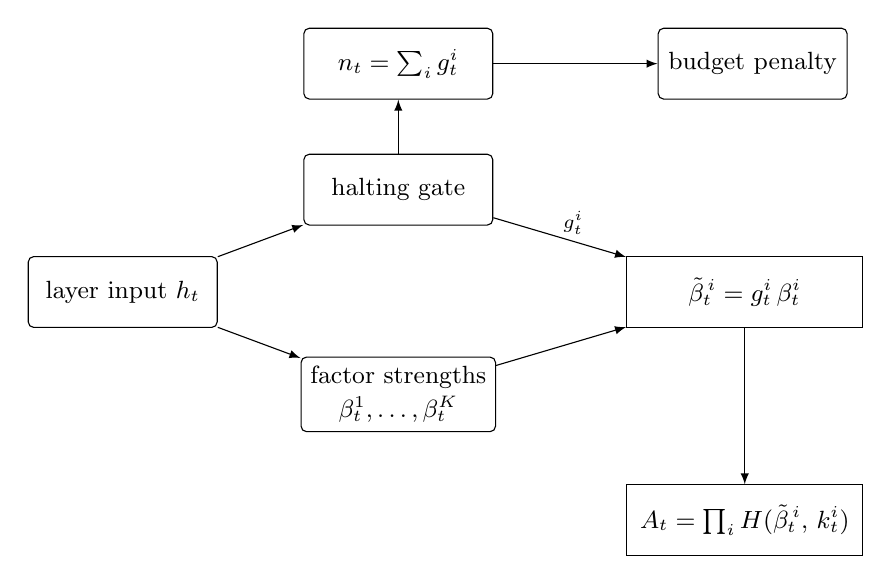
\begin{tikzpicture}[
		box/.style = {draw, rounded corners=2pt, minimum width=24mm, minimum height=9mm, align=center, font=\small},
		fac/.style = {draw, minimum width=30mm, minimum height=9mm, align=center, font=\small},
		>=latex
	]
	\node[box] (nt)   at (3.5,2.9)  {$n_t=\sum_i g_t^{i}$};
	\node[box] (bud)  at (8.0,2.9)  {budget penalty};
	\node[box] (gate) at (3.5,1.3)  {halting gate};
	\node[box] (h)    at (0,0)      {layer input $h_t$};
	\node[box] (beta) at (3.5,-1.3) {factor strengths\\[-2pt]$\beta_t^{1},\dots,\beta_t^{K}$};
	\node[fac] (mul)  at (7.9,0)    {$\tilde{\beta}_t^{\,i} = g_t^{i}\,\beta_t^{i}$};
	\node[fac] (prod) at (7.9,-2.9) {$A_t=\prod_i H(\tilde{\beta}_t^{\,i},\,k_t^{i})$};

	\draw[->] (h) -- (gate);
	\draw[->] (h) -- (beta);
	\draw[->] (gate) -- node[above right, font=\scriptsize, inner sep=1pt] {$g_t^{i}$} (mul);
	\draw[->] (beta) -- (mul);
	\draw[->] (mul) -- (prod);
	\draw[->] (gate) -- (nt);
	\draw[->] (nt) -- (bud);
	\end{tikzpicture}
	\caption{The adaptive-order layer. The halting gate emits monotone gates that scale the factor strengths; the sum of the gates is the token's effective order and is the quantity the budget penalty acts upon.}
	\label{fig:mechanism}
\end{figure}

\subsection{Training objective}

The layer is trained on the sum of the task loss and a penalty on the mean
effective order,
\begin{equation}
\mathcal{L} \;=\; \mathcal{L}_{\text{task}} \;+\; \gamma(s)\,\overline{n},
\qquad
\overline{n} \;=\; \frac{1}{BT}\sum_{b,t} n_{b,t},
\end{equation}
where $\gamma(s)$ is the budget weight at training step $s$. No term in this
objective references the correct allocation; the gate receives no supervision on
$n_t$ and must infer it from the interaction between the two terms, the task loss
opposing closure where expressivity is needed and the penalty favouring closure
everywhere else.

The gate is initialised open, so that at the first step the layer is exactly a
fixed-order model with $K = n_h$, which is the configuration known to converge.
The budget weight is held at zero for a warm-up period and then increased
linearly to its final value, so that the gate cannot close before the task has
been learned:
\begin{equation}
\gamma(s) \;=\;
\begin{cases}
0, & s \le s_{\text{warm}},\\[2pt]
\gamma \cdot \min\!\left(1, \dfrac{s - s_{\text{warm}}}{s_{\text{ramp}}}\right), & s > s_{\text{warm}} .
\end{cases}
\end{equation}
A configuration with $\gamma = 0$, in which the gate is present and trained but
never penalised, serves as the control for the effect of the gate's presence
alone.

\section{Cost Accounting and Execution Strategy}

The implementation evaluated here expands all $n_h$ factors and multiplies the
disabled ones by zero. This is numerically exact, and it is the strategy under
which every cost figure in this work is obtained. Accordingly, cost is reported
throughout as \emph{required work per token}, defined as the mean number of
factors whose gate is open at evaluation,
\begin{equation}
\text{cost} \;=\; \frac{1}{|\mathcal{T}|}\sum_{t \in \mathcal{T}} n_t ,
\end{equation}
where $\mathcal{T}$ ranges over positions carrying a group element, special
tokens being excluded because their correct transition is the identity. Under the
dense strategy a reduction in this quantity does not by itself reduce elapsed
time; converting it into elapsed time requires a ragged execution strategy in
which disabled factors are not materialised, and that is a subject of continuing
work.

\section{Experimental Design}
\label{sec:design}

\subsection{Data}

Sequences of length $k = 128$ are generated over a chosen alphabet of
permutations of five symbols, with the target at each position the cumulative
product of all symbols up to and including that position. Unless stated
otherwise, $100{,}000$ sequences are used for training and $2{,}000$ held out for
evaluation.

Two families of alphabet are used. The first is a mixture family, containing ten
transpositions and twenty-four five-cycles, in which a mixture parameter $p$
controls the fraction of five-cycles; the generated group is $S_5$ for every
$p < 1$, so the requirement is four for a five-cycle and one for a transposition,
and the expected requirement is $E[D] = 1 + 3p$. The second is a closure family,
in which the alphabet is varied so that the generated group changes while the
symbols themselves are held as similar as possible; this family operationalises
the prediction of Section \ref{sec:demand}, since alphabets of comparable size
fall on either side of the $A_5$/$S_5$ boundary.

\subsection{Model and optimisation}

All experiments use a single layer with twelve heads of dimension thirty-two and
hidden width $128$, in bfloat16. Optimisation is by AdamW at a constant learning
rate of $10^{-3}$, batch size $128$, for $20{,}000$ steps unless stated
otherwise. Experiments are run on an NVIDIA RTX 4050 Laptop GPU with 6\,GB of
memory.

\subsection{Arms and controls}

Three conditions are compared, and where they appear together they are trained
within a single invocation so that no comparison depends on a figure recorded
elsewhere.

\begin{enumerate}[label={(\arabic*)}]
	\item \textbf{Fixed order.} The unmodified layer at a constant $n_h$. Cost is
	$n_h$ by construction.
	\item \textbf{Oracle allocation.} The adaptive layer with gates supplied from
	ground truth, so that $n_t = D(g_t)$ exactly. This condition uses the same
	architecture and the same parameter count as the fixed-order arm at
	$n_h = 4$, differing only in the computation spent, and it establishes the
	best allocation attainable rather than the allocation a learned gate produces.
	\item \textbf{Learned allocation.} The adaptive layer with the halting gate
	trained under the budget penalty and no supervision on $n_t$.
\end{enumerate}

\subsection{Metrics}

Token accuracy is the fraction of positions predicted correctly. Sequence
accuracy requires every position of a sequence to be correct and is
correspondingly stricter: at $k = 128$, per-position accuracy of $0.99$
corresponds to sequence accuracy of $0.28$.

For the adaptive conditions, the allocation is evaluated against the requirement
$D$ of Equation \ref{eq:demand}, clipped to the factor count available. Three
quantities are reported. The mean absolute allocation error is
$\frac{1}{|\mathcal{T}|}\sum_t |n_t - D(g_t)|$. The under-allocated and
over-allocated fractions are reported separately rather than combined, since
under-allocation removes expressivity the task requires whereas over-allocation
only expends computation. Finally, the mean of $n_t$ is reported \emph{grouped by
the requirement} $D$, which distinguishes a gate that tracks the requirement from
one that reaches the same average by closing uniformly across all tokens.

\subsection{Measurement protocol}

The bfloat16 kernels used by the implementation employ non-deterministic atomic
accumulation, so repeated runs of an identical configuration are not bitwise
identical. On configurations that solve reliably this produces a spread of
approximately $0.005$ in token accuracy and $0.05$ in sequence accuracy. On the
configurations characterised in Section 4.6 the outcome distribution is bimodal
and the spread is far larger, with identical configurations producing token
accuracies of $0.1177$ and $0.9598$. On such configurations the summary statistic
reported is the fraction of runs that escape the loss plateau, taken over
repeated runs, rather than a mean.

Every experiment is accompanied by a self-test that evaluates its measurement
code against synthetic inputs whose correct output is known in advance, and each
such test is confirmed to fail when run against a deliberately incorrect
implementation.
\null

%====================================================Chapter 4===============================================================
\begin{center}
	\chapter{RESULTS AND ANALYSIS}
\end{center}
\justifying

\section{Baseline Reproduction}

The base architecture was rebuilt from the reference implementation and its
published state-tracking behaviour reproduced on the available hardware. On
$S_3$, the published contrast is recovered exactly: $n_h = 2$ reaches sequence
accuracy $1.000$ within a single epoch, while $n_h = 1$ remains at $0.000$,
consistent with the requirement of two factors for a three-cycle. On $S_5$ with
$n_h = 4$, trained on $500{,}000$ sequences for $100$ epochs, the model attains
token accuracy $0.864$ at sequence length $512$ after training at length $128$,
with whole-sequence accuracy perfect through position $121$. The length
extrapolation behaviour matches the published result qualitatively.

This baseline underlies every comparison reported below.

\section{Reachability of Permutation Transitions}

Every element of $S_5$ was reconstructed by explicit construction at every factor
count $K$ from zero to four, under a free $\beta$ and under $\beta$ held at $2$.
All $120$ elements were treated at each $K$, and the worst reconstruction error
over the entire set was $1.17 \times 10^{-15}$. Table \ref{table:reach} records
which combinations admit an exact representation.

\begin{table}[ht]
	\caption{Reachability of permutations of transposition length $\ell$ using $K$ factors. A tick denotes exact representation; a dash denotes that no exact representation exists.}
	\centering
	\begin{tabular}{c c c c c c | c c c c c}
		\hline\hline
		& \multicolumn{5}{c|}{Learnable $\beta \in [0,2]$} & \multicolumn{5}{c}{Fixed $\beta = 2$} \\
		$\ell$ & $K{=}0$ & $K{=}1$ & $K{=}2$ & $K{=}3$ & $K{=}4$ & $K{=}0$ & $K{=}1$ & $K{=}2$ & $K{=}3$ & $K{=}4$ \\ [0.5ex]
		\hline
		0 & \checkmark & \checkmark & \checkmark & \checkmark & \checkmark & \checkmark & --         & \checkmark & --         & \checkmark \\
		1 & --         & \checkmark & \checkmark & \checkmark & \checkmark & --         & \checkmark & --         & \checkmark & --         \\
		2 & --         & --         & \checkmark & \checkmark & \checkmark & --         & --         & \checkmark & --         & \checkmark \\
		3 & --         & --         & --         & \checkmark & \checkmark & --         & --         & --         & \checkmark & --         \\
		4 & --         & --         & --         & --         & \checkmark & --         & --         & --         & --         & \checkmark \\ [1ex]
		\hline
	\end{tabular}
	\label{table:reach}
\end{table}

The left half exhibits the rank bound alone: every $K \ge \ell$ is reachable. The
right half exhibits both bounds acting together, and the alternating pattern is
the determinant-parity constraint, under which exactly half of the admissible
combinations are lost. This result is what fixes the placement of the gate on the
factor strength rather than on a selection between fixed values, as described in
Section \ref{sec:mechanism}.

\section{Verification of the Order-Requirement Model}

The three-dimensional faithful representation of $A_5$ was constructed
independently from geometry, as the rotation group of the icosahedron, and
verified against the properties the model requires. The construction yields $60$
distinct rotations closed under composition with a closure error of
$1.4 \times 10^{-16}$; the element-order profile is
$\{1{:}1,\ 2{:}15,\ 3{:}20,\ 5{:}24\}$, which is that of $A_5$; and the
isomorphism is exhibited explicitly through the action on the five inscribed
octahedra, verified to be faithful, to have even image, and to be surjective onto
all $60$ elements. Every non-identity element of the representation has
$\operatorname{rank}(\rho(g) - I) = 2$, and each factors into exactly two
Householder reflections with a worst reconstruction error of
$1.31 \times 10^{-15}$.

Table \ref{table:a5} sets the resulting requirement against the transposition
length for each conjugacy class. The two quantities agree except on the
five-cycles, where they differ by a factor of two.

\begin{table}[ht]
	\caption{Transposition length and order requirement within $A_5$}
	\centering
	\begin{tabular}{P{4.2cm} c c c}
		\hline\hline
		Element type & Count & $\ell$ (permutation rep.) & $D$ (3-D rep.) \\ [0.5ex]
		\hline
		Identity & 1 & 0 & 0 \\
		Double transposition & 15 & 2 & 2 \\
		Three-cycle & 20 & 2 & 2 \\
		Five-cycle & 24 & 4 & 2 \\ [1ex]
		\hline
	\end{tabular}
	\label{table:a5}
\end{table}

\section{Alphabet Closure as a Predictor of Trainability}

Section \ref{sec:demand} predicts that the generated group, rather than the
alphabet size or the identity of the individual symbols, determines the required
factor count. The prediction was tested by holding the factor count at
$n_h = 3$, one below the requirement of $S_5$ and one above the requirement of
$A_5$, and varying the alphabet across the closure boundary. Under the
order-requirement model, alphabets generating $A_5$ should be solvable at this
factor count and alphabets generating $S_5$ should not, irrespective of their
size. Table \ref{table:closure} reports the outcome.

\begin{table}[ht]
	\caption{Trainability at $n_h = 3$ as a function of the group generated by the alphabet}
	\centering
	\begin{tabular}{P{6.0cm} c c}
		\hline\hline
		Alphabet & Generated group & Token accuracy \\ [0.5ex]
		\hline
		24 five-cycles & $A_5$ & 0.9991 \\
		\quad + 15 double transpositions & $A_5$ & 0.9994 \\
		\quad + 20 three-cycles (44 symbols) & $A_5$ & 0.9952 \\
		\quad + 1 transposition (25 symbols) & $S_5$ & 0.1094 \\
		\quad + 10 transpositions (34 symbols) & $S_5$ & 0.0307 \\ [1ex]
		\hline
	\end{tabular}
	\label{table:closure}
\end{table}

The separation follows the generated group exactly. Alphabet size is ruled out as
the operative variable in both directions: the largest alphabet, with $44$
symbols, is the easiest arm, while a $25$-symbol alphabet differing from a
solvable one by the addition of a single transposition fails. This is the
behaviour predicted by Equation \ref{eq:demand} and is not reproducible by any
model in which difficulty is an attribute of the individual symbol. Each cell of
this grid is a single training run; repetition of the grid under the protocol of
Section 4.6 is in progress.

\section{Capability at Matched Computation}

The mixture family was used to compare fixed orders against the oracle allocation
at equal parameter count. Table \ref{table:matched} reports the full sweep at
$p = 0.10$, and Figure \ref{fig:matched} plots accuracy against required work per
token for the same configuration.

\begin{table}[ht]
	\caption{Token accuracy against required work per token, mixture parameter $p = 0.10$}
	\centering
	\begin{tabular}{P{3.6cm} c c}
		\hline\hline
		Condition & Cost per token & Token accuracy \\ [0.5ex]
		\hline
		Fixed, $n_h = 1$ & 1.000 & 0.1583 \\
		Fixed, $n_h = 2$ & 2.000 & 0.4659 \\
		Fixed, $n_h = 3$ & 3.000 & 0.9696 \\
		Fixed, $n_h = 4$ & 4.000 & 0.9999 \\
		Oracle allocation & \textbf{1.300} & \textbf{0.9999} \\ [1ex]
		\hline
	\end{tabular}
	\label{table:matched}
\end{table}

\begin{figure}[ht]
	\centering
	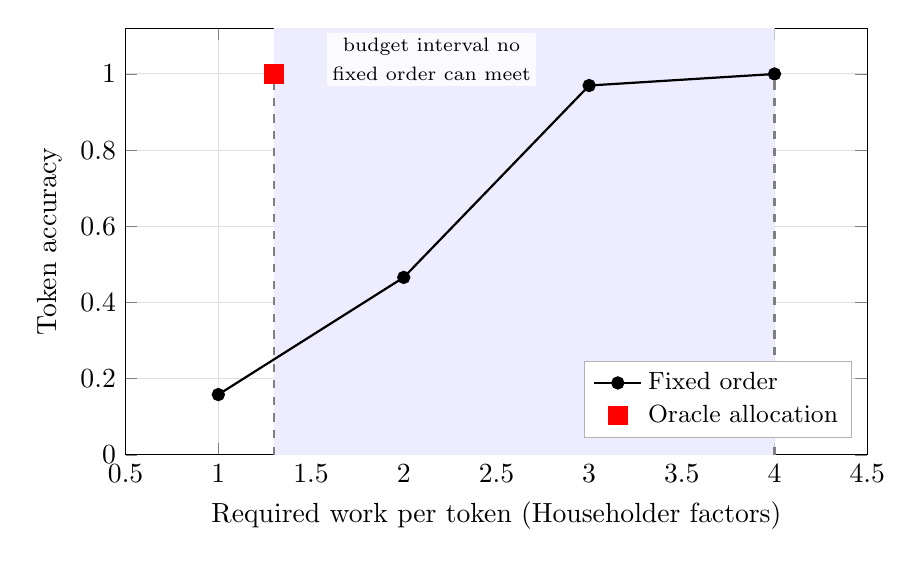
\begin{tikzpicture}
	\begin{axis}[
		width=11cm, height=7cm,
		xlabel={Required work per token (Householder factors)},
		ylabel={Token accuracy},
		xmin=0.5, xmax=4.5, ymin=0, ymax=1.12,
		grid=major, grid style={gray!25},
		legend style={at={(0.98,0.04)}, anchor=south east, draw=gray!60, fill=white, font=\small},
		legend cell align={left},
		every axis plot/.append style={thick},
	]
	\addplot[draw=none, fill=blue!7, forget plot] coordinates {
		(1.300,0) (4.0,0) (4.0,1.12) (1.300,1.12)
	} \closedcycle;
	\node[font=\scriptsize, align=center, anchor=north, fill=white, fill opacity=0.75,
	      text opacity=1, inner sep=2pt] at (axis cs:2.15,1.11)
		{budget interval no\\ fixed order can meet};
	\addplot[mark=*, color=black] coordinates {
		(1.0,0.1583) (2.0,0.4659) (3.0,0.9696) (4.0,0.9999)
	};
	\addlegendentry{Fixed order}
	\addplot[only marks, mark=square*, mark size=3.2pt, color=red] coordinates {
		(1.300,0.9999)
	};
	\addlegendentry{Oracle allocation}
	\addplot[dashed, color=gray, forget plot] coordinates {(1.300,0) (1.300,0.9999)};
	\addplot[dashed, color=gray, forget plot] coordinates {(4.0,0) (4.0,0.9999)};
	\end{axis}
	\end{tikzpicture}
	\caption{Accuracy against required work at $p = 0.10$. The oracle allocation attains the accuracy of the $n_h = 4$ model at $1.300$ factors per token. No fixed order occupies the interval between these two points, because the fixed order is integer-valued.}
	\label{fig:matched}
\end{figure}

Table \ref{table:sweep} extends the comparison across three mixture rates. In
each case the oracle allocation matches the accuracy of the cheapest fixed order
that solves the task, at a fraction of the required work.

\begin{table}[ht]
	\caption{Oracle allocation against the cheapest adequate fixed order}
	\centering
	\begin{tabular}{c c c c c}
		\hline\hline
		$p$ & $E[D]$ & Fixed $n_h{=}4$ & Oracle allocation & Reduction \\ [0.5ex]
		\hline
		0.05 & 1.150 & 0.9999 at cost 4 & 1.0000 at cost 1.150 & $3.48\times$ \\
		0.10 & 1.300 & 0.9999 at cost 4 & 0.9999 at cost 1.300 & $3.08\times$ \\
		0.25 & 1.752 & 0.9997 at cost 4 & 0.9999 at cost 1.752 & $2.29\times$ \\ [1ex]
		\hline
	\end{tabular}
	\label{table:sweep}
\end{table}

Because a fixed order is integer-valued, it occupies only the discrete points
$1, 2, 3, 4$ on the cost axis. For any computational budget $B$ satisfying
$E[D] \le B < D_{\max}$, no fixed-order model both meets the budget and solves
the task, whereas an adaptive model does. The width of that interval narrows as
$p$ increases, in agreement with $E[D] = 1 + 3p$.

Two properties of these figures govern their interpretation. The oracle condition
is a control in which the correct per-token order is supplied from ground truth;
it establishes the reduction attainable by a correct allocation and is
independent of whether a gate can learn that allocation. The reduction is in
required work per token and not in elapsed time: under the dense execution
strategy of Section 3.5 the adaptive condition ran in $756$\,s against $761$\,s
for the full-cost condition, a difference within measurement noise, because
disabled factors are still materialised and multiplied by zero.

\section{Training Stability and Its Consequences for Measurement}

Fifty training runs of the unmodified architecture were conducted across four
alphabets at $20{,}000$ steps with a constant learning rate, with the data held
fixed and only the run varied. Table \ref{table:census} reports the outcome.

\begin{table}[ht]
	\caption{Escape fraction over repeated runs of identical configurations}
	\centering
	\begin{tabular}{P{4.0cm} c c P{3.0cm}}
		\hline\hline
		Configuration & Escapes / runs & Rate & Outcome distribution \\ [0.5ex]
		\hline
		$A_5$ five-cycles, $n_h{=}2$ & 4 / 14 & 0.29 & bimodal \\
		$A_5$ with double transp., $n_h{=}2$ & 2 / 10 & 0.20 & bimodal \\
		$A_5$ with double transp., $n_h{=}4$ & 1 / 10 & 0.10 & bimodal \\
		$S_5$ with transposition, $n_h{=}4$ & 3 / 10 & 0.30 & bimodal \\ [1ex]
		\hline
	\end{tabular}
	\label{table:census}
\end{table}

Outcomes on these configurations are bimodal. A run either escapes the loss
plateau and reaches approximately $0.99$ token accuracy, or remains at chance
accuracy near $0.04$; intermediate outcomes are rare. Escape is abrupt, with the
loss falling by two orders of magnitude within a single logging interval, and
occurs anywhere between step $5{,}000$ and step $20{,}000$. Non-determinism in the
bfloat16 kernels alone is sufficient to select between the two outcomes: an
identical configuration under an identical seed has produced both.

Two consequences follow. The first is methodological: a single run of such a
configuration carries no information about the configuration, and the appropriate
summary statistic is the escape fraction over repeated runs. Distinguishing an
escape rate of $0.25$ from one of $0.75$ at the $5\%$ level with $80\%$ power
requires approximately $20$ runs per condition, which is the budget adopted for
subsequent experiments on these configurations. Under the measured rates, the
best run obtained on the $S_5$ alphabet reaches token accuracy $0.9994$ and
sequence accuracy $0.9415$, with accuracy $0.9995$ on even targets and $0.9994$
on odd, establishing that the configuration is solvable and that the difficulty
is one of optimisation rather than expressivity.

The second consequence concerns the scope of the proposed mechanism. Table
\ref{table:benefit} sets the measured escape rates against the reduction that a
correct allocation would deliver on each configuration.

\begin{table}[ht]
	\caption{Available reduction against training reliability}
	\centering
	\begin{tabular}{P{3.6cm} P{4.2cm} P{3.0cm}}
		\hline\hline
		Available reduction & Configurations & Trains reliably \\ [0.5ex]
		\hline
		$2.29\times$ -- $3.48\times$ & $p = 0.05,\ 0.10,\ 0.25$ & yes, $\ge 0.9997$ \\
		$1.28\times$ & $S_5$ with transposition & 3 / 10 \\
		$1.00\times$ & $A_5$ alphabets & 1--4 / 10 \\ [1ex]
		\hline
	\end{tabular}
	\label{table:benefit}
\end{table}

Every configuration that trains reliably is one in which adaptive allocation
reduces required work by a factor between $2.3$ and $3.5$. Every configuration
that trains unreliably is one in which the available reduction is $1.28\times$ or
less, and for the $A_5$ alphabets it is exactly unity, since the requirement is
constant across the alphabet and no allocation can improve on a fixed order. The
region in which the architecture is least stable and the region in which the
proposed mechanism is useful are therefore disjoint.

\section{Error Characterisation}

The structure of the errors made by under-provisioned models was examined at
$p = 0.10$. Table \ref{table:forensics} reports the results.

\begin{table}[ht]
	\caption{Error structure at $p = 0.10$}
	\centering
	\begin{tabular}{P{4.6cm} c c c}
		\hline\hline
		& $n_h{=}1$ & $n_h{=}3$ & $n_h{=}4$ \\ [0.5ex]
		\hline
		Token / sequence accuracy & 0.1822 / 0.0000 & 0.9740 / 0.7145 & 0.9999 / 0.9940 \\
		Per-high-requirement-token success & 0.7124 & 0.9947 & 1.0000 \\
		Mean error-run length & 30.13 & 2.00 & 1.11 \\
		Sequences containing any error & 2000 / 2000 & 571 / 2000 & 12 / 2000 \\ [1ex]
		\hline
	\end{tabular}
	\label{table:forensics}
\end{table}

Errors are clustered rather than independent, and they are not absorbing. Two
models of the error process were stated in advance and are both inconsistent with
the measurements: independent per-position errors predict a sequence accuracy of
$0.974^{128} = 0.034$ for the $n_h = 3$ model against $0.7145$ observed, while
permanent corruption of the state predicts a token accuracy of $0.746$ against
$0.9740$ observed. The $n_h = 3$ model recovers from errors, with a median
error-run length of a single position. Since a corrupted group-tracking state
possesses no mechanism by which to correct itself, information sufficient for
recovery is being carried outside the transition matrices, and the additive
channel of the recurrence is the natural candidate.

\section{End-to-End Training of the Halting Gate}

The learned condition was evaluated at $p = 0.10$ against the fixed-order and
oracle conditions, at four budget weights $\gamma \in \{0,\ 0.01,\ 0.03,\ 0.1\}$
and three random seeds, giving $18$ training runs conducted within a single
invocation. The budget penalty was held at zero for $4{,}000$ steps and then
increased linearly over a further $4{,}000$. Gates were evaluated in hard mode,
so every reported cost is an integer factor count.

In one of the three seeds the gate converged to the oracle allocation. Table
\ref{table:gate} reports that seed.

\begin{table}[ht]
	\caption{Learned allocation against the oracle, for the seed in which the gate converged}
	\centering
	\begin{tabular}{P{3.4cm} c c c c c}
		\hline\hline
		Condition & Token & Sequence & Cost & Mean abs.\ error & Correlation \\ [0.5ex]
		\hline
		Fixed, $n_h = 4$ & 0.9998 & 0.9885 & 4.000 & --- & --- \\
		Oracle allocation & 0.9996 & 0.9770 & 1.298 & 0.00 & 1.00 \\
		Learned, $\gamma = 0.03$ & 0.9999 & 0.9910 & \textbf{1.298} & \textbf{0.00} & \textbf{1.00} \\
		Learned, $\gamma = 0.1$ & 1.0000 & 0.9970 & \textbf{1.298} & \textbf{0.00} & \textbf{1.00} \\ [1ex]
		\hline
	\end{tabular}
	\label{table:gate}
\end{table}

The mean absolute allocation error of zero is taken over $256{,}000$ evaluated
tokens. The decisive measurement is the allocation grouped by requirement, shown
in Figure \ref{fig:alloc}, since a gate that reached the correct average by
closing uniformly across all tokens would produce the same mean cost while
carrying no information. Every token of requirement one received exactly one
factor and every token of requirement four received exactly four, matching the
oracle in both groups. Two independent budget weights produced the same
allocation. The differences in accuracy relative to the oracle lie within the
noise floor established in Section 3.7.

\begin{figure}[ht]
	\centering
	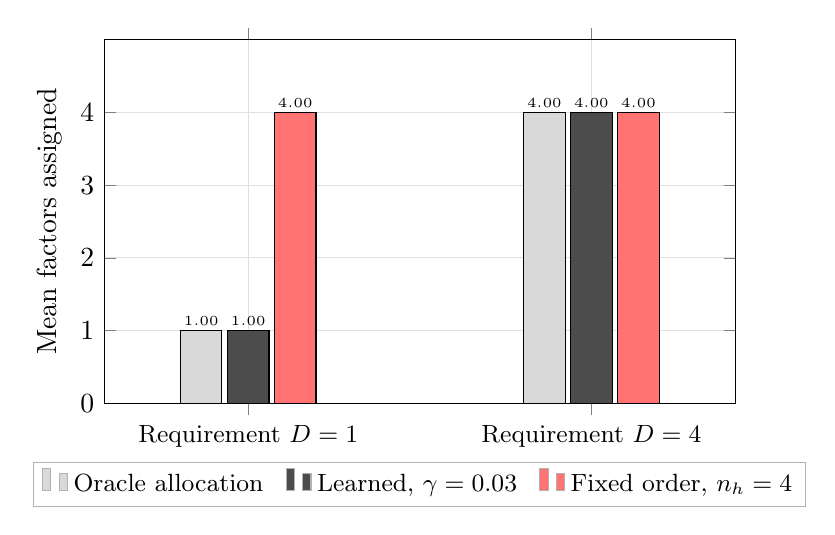
\begin{tikzpicture}
	\begin{axis}[
		width=9.6cm, height=6.2cm,
		ybar,
		bar width=15pt,
		symbolic x coords={D1, D4},
		enlarge x limits=0.42,
		xtick=data,
		xticklabels={Requirement $D=1$, Requirement $D=4$},
		xticklabel style={font=\small},
		ymin=0, ymax=5.0,
		ytick={0,1,2,3,4},
		ylabel={Mean factors assigned},
		legend style={at={(0.5,-0.16)}, anchor=north, legend columns=3,
		              draw=gray!60, font=\small, /tikz/every even column/.append style={column sep=6pt}},
		legend cell align={left},
		grid=major, grid style={gray!25},
		nodes near coords={\pgfmathprintnumber[fixed, zerofill, precision=2]{\pgfplotspointmeta}},
		nodes near coords style={font=\tiny, inner sep=1.5pt},
	]
	\addplot[fill=gray!30] coordinates {(D1, 1.00) (D4, 4.00)};
	\addlegendentry{Oracle allocation}
	\addplot[fill=black!70] coordinates {(D1, 1.00) (D4, 4.00)};
	\addlegendentry{Learned, $\gamma = 0.03$}
	\addplot[fill=red!55] coordinates {(D1, 4.00) (D4, 4.00)};
	\addlegendentry{Fixed order, $n_h = 4$}
	\end{axis}
	\end{tikzpicture}
	\caption{Mean number of factors assigned, grouped by the token's requirement, over $230{,}531$ tokens of requirement one and $25{,}469$ of requirement four. The learned allocation is indistinguishable from the oracle in both groups, while the fixed-order model spends four factors on every token regardless of requirement.}
	\label{fig:alloc}
\end{figure}

In the remaining two seeds the gate did not depart from full order, holding cost
at exactly $4.000$ at every budget weight including the largest, with correlation
$0.00$ against the requirement. Across the three seeds the gate therefore
converged to the oracle allocation in one, and this is reported as a fraction in
accordance with the protocol of Section 3.7 rather than as a mean over seeds.

Two further observations bear on this outcome. First, task accuracy lies between
$0.98$ and $1.00$ in all eighteen runs, including those in which the gate did not
close; the variability is confined to the allocation and is independent of the
accuracy bimodality characterised in Section 4.6. Second, in the $\gamma = 0$
control, in which the gate is present but never penalised, the converging seed
still reached cost $3.369$ with correlation $0.43$, assigning a mean of $3.30$
factors to requirement-one tokens against $4.00$ to requirement-four tokens,
while the remaining seeds held at $4.000$. The task loss alone therefore exerts
pressure towards closure on low-requirement tokens, and the difference between
seeds is established before the budget penalty takes effect.

\section{Discussion}

The results divide into three groups, and the distinctions between them are
material to their interpretation.

The reachability bounds and the order-requirement model are established by
explicit construction in double-precision arithmetic, with no optimiser involved,
and hold independently of any training outcome. The closure experiment provides
the corresponding empirical confirmation, separating perfectly along the
predicted variable while excluding alphabet size as an alternative explanation.

The matched-computation results establish what a correct per-token allocation
achieves: accuracy equal to the cheapest adequate fixed order at $2.29$ to $3.48$
times less required work, across three mixture rates. Because the allocation in
this condition is supplied from ground truth, these figures bound the attainable
reduction rather than demonstrate that it is attainable by a learned mechanism.

The end-to-end results address that remaining question directly. A gate trained
under a penalty on expected computation, receiving no supervision on the
allocation, reproduced the oracle allocation exactly in one of three seeds,
assigning the correct integer factor count to every one of $256{,}000$ evaluated
tokens. The allocation was recovered rather than approximated, and it was
recovered at two independent budget weights. Establishing the conditions under
which this outcome occurs reliably is the principal objective of the continuing
work described in Chapter 5.

A final observation concerns the interaction between Sections 4.5 and 4.6. The
configurations on which the architecture trains least reliably are precisely
those on which adaptive allocation offers a reduction of $1.28\times$ or less,
while every configuration offering a reduction above $2.29\times$ trains to
$0.9997$ or better. The instability of the base architecture and the operating
region of the proposed mechanism therefore do not overlap, which bounds the
extent to which the former limits the latter.
\null

%===================================================Chapter5=================================================================
\begin{center}
	\chapter{CONCLUSIONS AND FUTURE WORK}
\end{center}
\justifying

\section{Conclusions}

This work addressed the allocation of computation in linear recurrent layers
whose state-transition operator is a product of generalized Householder factors,
where the number of factors per token is conventionally a global hyperparameter.

The principal result is an order-requirement model for such layers. The number of
factors a symbol requires is determined by the minimum, over all faithful
representations of the group generated by the entire alphabet, of the rank of the
symbol's deviation from the identity. This quantity is not an attribute of the
symbol: a five-cycle requires four factors when the alphabet generates the
symmetric group $S_5$ and two when it generates the alternating group $A_5$,
because the latter admits a three-dimensional faithful representation as the
rotation group of the icosahedron. The model was verified by constructing that
representation from geometry and confirming every property it depends upon, with
a worst reconstruction error of $1.31 \times 10^{-15}$. Its central prediction,
that the generated group rather than the alphabet size governs the required
order, was confirmed experimentally: at a fixed factor count of three, alphabets
generating $A_5$ reach token accuracies between $0.9952$ and $0.9994$ while
alphabets generating $S_5$ reach $0.1094$ and $0.0307$, with the largest alphabet
tested falling in the former group and one of the smallest in the latter.

Two reachability bounds were established by explicit construction over all $120$
elements of $S_5$ at every factor count. The rank bound requires the factor count
to be at least the transposition length of the target. The determinant-parity
bound shows that when the factor strength is held at its reflection value, only
factor counts congruent to the transposition length modulo two admit an exact
representation, so that half of all targets are unreachable at any given count.
This second bound is not a peripheral observation: it determines that a mechanism
varying the effective order must scale a learnable factor strength toward zero
rather than select among fixed values, and the architecture proposed here is
constructed accordingly.

The practical significance of the order-requirement model is that it renders the
factor count a hyperparameter that cannot be selected reliably by inspection.
Setting it correctly requires the minimum faithful representation dimension of
the group generated by the data, which changes discontinuously as the alphabet
changes and is not observable from a dataset. A layer that infers its own order
therefore removes a hyperparameter that has no reliable manual setting, and this
argument is independent of any reduction in computation.

On the mechanism itself, an adaptive-order layer was implemented in which a
monotone halting gate assigns a per-token factor count and is trained under a
penalty on expected computation with no supervision on the allocation. Under an
oracle allocation supplied from ground truth, the layer attains the accuracy of
the cheapest adequate fixed order at $1.150$, $1.300$ and $1.752$ factors per
token where that fixed order costs four, corresponding to reductions in required
work of $3.48\times$, $3.08\times$ and $2.29\times$. Trained end to end across
three random seeds, the halting gate reproduced this allocation exactly in one
seed, assigning one factor to every requirement-one token and four to every
requirement-four token across $256{,}000$ evaluated tokens, at two independent
budget weights. The allocation was recovered rather than approximated.

A supporting result concerns measurement. Across fifty training runs, outcomes on
the harder alphabets were found to be bimodal rather than concentrated, with
escape from the loss plateau occurring in between $10\%$ and $30\%$ of runs and
selected by kernel non-determinism alone. The appropriate summary statistic on
such configurations is the escape fraction over repeated runs, and approximately
twenty runs per condition are required to distinguish escape rates of practical
interest. Setting these rates against the reduction available on each
configuration establishes that the configurations offering reductions above
$2.29\times$ train reliably, while those that train unreliably offer $1.28\times$
or less, so that the instability of the base architecture and the operating
region of the proposed mechanism are disjoint.

Two limitations bound the scope of these conclusions. All reductions reported
here are in required work per token, measured under a dense execution strategy in
which disabled factors are materialised and multiplied by zero; the adaptive and
full-cost conditions differ in elapsed time by less than one percent, and no
reduction in elapsed time is claimed. And the end-to-end allocation result rests
on three seeds at a single operating point on a single task family.

\section{Future Work}

\subsection{Reliability of the learned allocation}

The immediate objective is to establish the conditions under which the halting
gate converges to the correct allocation reliably. The evidence points to the
gate's initialisation rather than to the strength of the budget penalty: at the
largest penalty weight tested, the non-converging seeds held cost at exactly the
full factor count rather than at an intermediate value, which indicates a gate
that is not responding to the penalty rather than one responding insufficiently.
Two properties of the initialisation are relevant. The output weight of the gate
network is initialised at zero, which makes the gate constant with respect to its
input until that weight moves, so that the gate can raise or lower one global
order but cannot allocate. And the output bias places the halting nonlinearity at
a point where its derivative is small, attenuating the gradient that would move
that weight. Both are addressed by parameters now exposed for controlled study:
the initialisation bias of the gate, and a learning rate applied to the gate
independently of the remainder of the model. These will be evaluated one at a
time over ten seeds per condition, under the measurement protocol of Section 3.7.

\subsection{Inference of the order requirement from data}

A sharper form of the order-requirement model can be tested once the allocation
is reliable. The requirement for a five-cycle differs between an $A_5$ alphabet
and an $S_5$ alphabet, yet the symbol itself is identical in both. A gate that
assigns two factors under the first and four under the second would be inferring
a global algebraic property of the alphabet from purely local statistics, which
constitutes a considerably stronger result than a correlation between the
allocation and a measure of difficulty.

\subsection{Ragged execution and elapsed-time measurement}

Converting the measured reduction in required work into a reduction in elapsed
time requires an execution strategy in which disabled factors are not
materialised. Implementing this, and benchmarking it both at batch size one and
at the batch sizes typical of training, is the work that would substantiate the
efficiency argument. The benchmark is to be conducted in a manner that admits the
outcome that batching absorbs the saving, which is a possible and informative
result.

\subsection{Generality across groups and tasks}

The order-requirement model is stated for arbitrary finite groups, but has been
verified empirically within $S_5$ and $A_5$. Extending the empirical
verification to $S_3$, $S_4$ and $A_4$ would confirm that the model predicts the
required factor count across groups rather than within a single one. Beyond the
permutation setting, evaluation on a state-tracking task not designed for this
study, such as tracking board configurations in a two-player game, would
establish whether the mechanism transfers to tasks whose state structure is not
a group word problem by construction.

\subsection{Consolidation of the experimental record}

Several results reported here rest on a single training run per condition,
specifically the closure grid of Section 4.4, the matched-computation sweep of
Section 4.5, and the error characterisation of Section 4.7. Repetition of these
under the protocol of Section 3.7, with the number of runs reported alongside
each figure, is scheduled before the final evaluation. A broader survey of the
linear-attention and state-space literature is to be completed over the same
period.
\null


\bibliographystyle{unsrt}
\bibliography{ref.bib}
\newpage


\end{document}